\documentclass[hidelinks, 12pt]{article}

\usepackage{subcaption}
\usepackage{comment}
\usepackage{caption}
\usepackage{fullpage}
\usepackage[utf8]{inputenc}
\usepackage{appendix}
\usepackage{amssymb}
\usepackage{amsmath}
\usepackage{hyperref}
\usepackage{float}
\usepackage{graphicx}
\graphicspath{ {./images/} }

\parskip = \baselineskip
\setlength{\parindent}{0pt}

\title{Pareto Replicating Theta Vaults}

\author{Mike Wu, Will McTighe \\ \small\texttt{\{mike, will\}@paretolabs.xyz}}

\date{February 2022}

\begin{document}

\maketitle

\tableofcontents

\begin{abstract}
Theta Vaults are a simple on-chain automated structured product that sells rolling weekly out-the-money option strategies with premiums returned to vault depositors as yield. The first implementation was selling covered calls, in which upside volatility is exchanged for yield.
Traditionally, Theta Vaults face two main challenges: first, the yield is capped by the efficiency of a matching process to find options buyers; second, they require oracles for liquidation which can introduce unwanted vulnerabilities.
In this paper, we present a design for Theta Vaults built on top of replicating market makers (RMMs), an extension of automated market makers that replicates a Black-Scholes covered call payoff.
We show this ``Replicating Theta Vault'', or RTV design precisely addresses the stated challenges.
Beyond covered calls, an ecosystem of efficient and secure options vaults can be built by a similar replication technique.
% I'm not sure that Ribbon requires an Oracle, it depends if Opyn's oTokens do, I need to check this.
\end{abstract}

\section{Preface}

This paper is a technical introduction to Pareto Replicating Theta Vaults, a redesign of the yield instrument popularized by Ribbon Finance, ThetaNuts, Friktion, among many others. We describe how to construct Theta Vaults on top of replicating market makers (RMMs), in which selling a covered call is equivalent to being a liquidity provider for an AMM. Our primary hypothesis is that the ability of RMMs to replicate a wide array of structured products can be used to design an options ecosystem with token composability as a first-class citizen. For Theta Vaults, RMMs offer a permission-less and auction-free solution that users may find attractive. In the following sections, we provide background information then present the mechanism underlying the Replicating Theta Vault (RTV).

The alpha product for Pareto RTVs is currently under development. Please reach out to \texttt{team@paretolabs.xyz} if you have any questions.

\section{Background}

We provide an overview of concepts required to understand RTVs. We offer a high-level explanation and leave a more mathematical treatment to the cited work.

\subsection{Constant Function Market Makers}

Constant function market makers (CFMMs) are a family of automated market makers (AMMs) used as token swap mechanisms on public blockchains. Liquidity providers (LPs) lend a token pair (e.g. Ethereum and USDC) to a supply of reserves managed by a smart contract. Users wishing to swap tokens can call the smart contract, paying a small fee that is rewarded to the LPs. However, the contract is programmed to ensure that a function of the token reserves remains constant, hence the name ``constant function''. This function is called the trading function or the invariant and defines the relative price of the two assets.

To introduce the notation we use throughout this paper, let $x, y \in \mathbf{R}_+$ be reserves for two tokens X and Y, and $\psi: \mathbf{R} \times \mathbf{R} \rightarrow \mathbf{R}$ be an invariant. For a fixed level of liquidity, we have $\psi(x, y) = k$ for a constant $k \in \mathbf{R}$. A trade of $\Delta x$ of token X for $\Delta y$ of token Y is allowed if and only if $\psi(x - \Delta x, y + \Delta y) = k$ for the same value $k$. For any CFMM, the (marginal) price of token Y in token X is a function of the reserves:
\[S(x) = \left(-\frac{dy}{dx}\right).\]
A common invariant is the product of the two reserves ($\psi = x\cdot y$), used by Uniswap \cite{angeris2019analysis,adams2021uniswap} and Balancer \cite{martinelli2019non} among others.
In this case, the marginal price is simply $\left(\frac{y}{x}\right)$.
Other invariants include the arithmetic sum ($\psi = x + y$) along with more complex ``mixtures'' of sum and product invariants such as Yieldspace \cite{niemerg2020yieldspace} or Curve \cite{egorov2021automatic}.

CFMMs and the broader class of AMMs, stand as an alternative to more traditional orderbook markets that require matching between buyers and sellers at various prices. CFMMs require no middlemen, expose transparent prices, have efficiency benefits as trades execute immediately, are oracle-free and hence less vulnerable to malicious actors, and are more robust under black-swan events \cite{chitra2021liveness}. Due to these advantages, CFMMs have grown to dominate the on-chain swap market, with Uniswap being the largest DEX and fourth largest exchange.
% Much more can be said about CFMMs, including impermanent loss and the structure of trading fees, but for this discussion, we recommend reading \cite{angeris2019analysis}.

\subsection{Replicating Market Makers}
\label{sec:rmm}

Given a CFMM with a specific invariant, what is the payoff to its liquidity providers? Generally, given $x$ units of a token valued at price $p_x$ on some reference market, my payoff is simply what I can sell my assets for. In this case,  $p_x \cdot x$. Given two tokens with $x$ units of X and $y$ units of Y, we can write the total payoff as:
\[V(p_x, p_y) = p_x\cdot x + p_y \cdot y = p_x (x + S(x)\cdot y_\psi(x))\]
where $S(x)$ is the marginal price and the notation $y_\psi(x)$ represents solving for $y$ in terms of $x$ with respect to the invariant $\psi$.
Altogether, $S(x)\cdot y_\psi(x)$ is the amount of token X we can get for $y$ units of token Y in the CFMM.
As we can see in Figure~\ref{fig:ammpayoff} below, the product invariant has a payoff function that suffers from divergence loss \cite{angeris2019analysis}. If the price does not deviate too much from the initial price that a liquidity provider (LP) deposited tokens at, the LP makes a profit vs. just holding the underlying asset. However, if the price changes a lot, the LP loses money that scales with the magnitude of the price change. For LPs with a directional belief in the token price, such a payoff is not optimal.

\begin{figure}[h!]
    \centering
    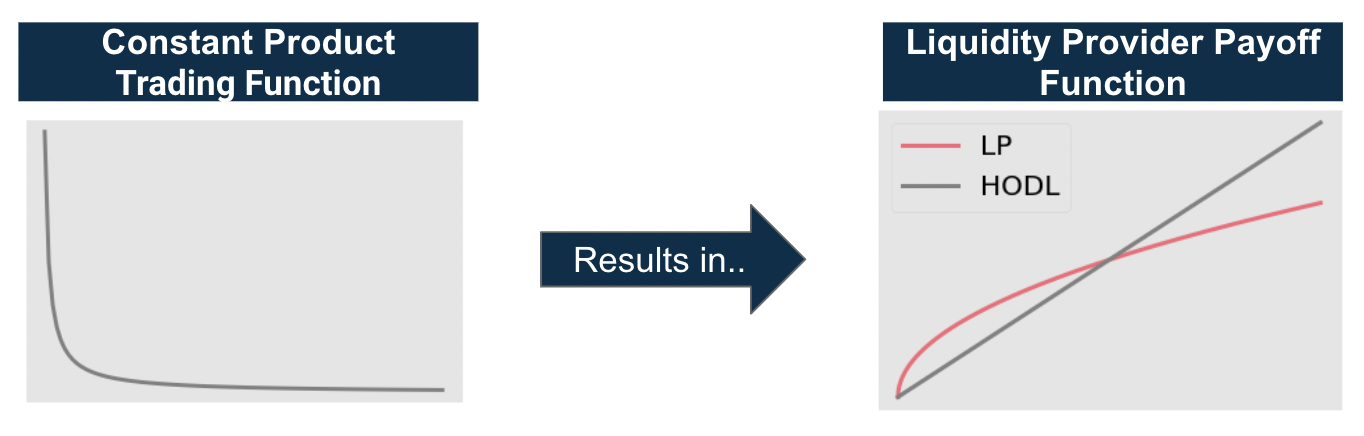
\includegraphics[width=0.8\linewidth]{ammpayoff.png}
    \caption{Automated Market Makers: Constant Product Invariant and Liquidity Provider Payoff Function. The CPMM trading function is $xy = k$ where $k$ is the invariant. The payoff function for a liquidity provider of this market can be simplified to $V(S) = 2\sqrt{Sk}$.}
    \label{fig:ammpayoff}
\end{figure}

This begs the question: given a desired LP payoff function, what is the corresponding invariant to achieve that payoff function? We can imagine all kinds of interesting payoff functions that might be attractive to LPs seeking to hedge or take on risk.  Above, we showed how to derive a payoff function $V$ from an invariant $\psi$. "Replicating Market Makers" (RMMs) showed us how to do the opposite, that is derive an invariant from a payoff function.

RMMs \cite{angeris2021replicating} show that for all payoff functions $V$ that are non-negative, concave, and 1-homogenous (this final condition is the strictest), one can derive an invariant by solving a convex optimization problem,
\[ \psi_V(x, y) = \inf_{p_x, p_y} \{ p_x \cdot x + p_y \cdot y - V(p_x, p_y) \}. \]
The method goes further to show that the payoff function and the invariant are Fenchel conjugates of one another. So, to enable LPs to achieve a payoff $V$, one can design a CFMM with the invariant $\psi_V$. We say that $\psi_V$ ``replicates'' the payoff $V$. The first RMM implementation, a liquidity provider payoff function that replicates the covered call options selling strategy is used to derive a corresponding trading function, as shown in Figure~\ref{fig:rmmpayoff}.

\begin{figure}[h!]
    \centering
    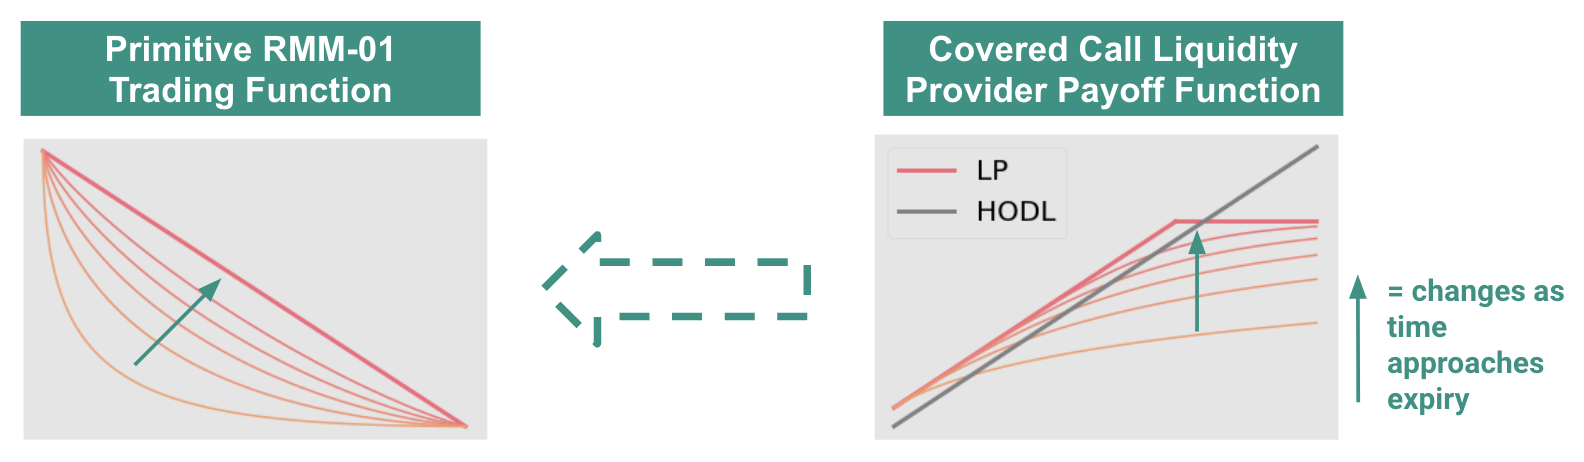
\includegraphics[width=0.8\linewidth]{rmmpayoff.png}
    \caption{Example of a Replicating Market Maker: RMM-01 Invariant and Liquidity Provider Payoff Function. The RMM-01 trading function is $y - K\Phi(\Phi^{-1}(1-x) - \sigma\sqrt{\tau} = k$ where $k$ is  the invariant, $K$ the strike price, $\sigma$ the implied volatility, $\tau$ the time to maturity, and $\Phi$ a Gaussian CDF.
    The RMM-01 Liquidity Provider payoff function is $V(S) = S(1-\Phi(d_1)+K\Phi(d_2))$ where $d_1 = \frac{\log(S/K) + (\sigma^2/2)\tau}{\sigma\sqrt{\tau}}$, $d_2 = d_1 - \sigma\sqrt{\tau}$.}
    \label{fig:rmmpayoff}
\end{figure}

\subsection{Options Review}
\label{sec:options}

We review the basics of a covered call. An option is a derivative instrument, which gives the owner the right to buy or sell an underlying asset at a pre-determined price (its strike price). The buyer of an option pays a premium to the seller in exchange for that right.

A \textit{call} option is an option with the right to buy an asset at a pre-determined ``strike price'' such that if the underlying asset price (also called the spot price) is above the strike, then the buyer may ``exercise'' the option, meaning purchase the underlying asset at the strike price. Critically, this is less than the spot price meaning the buyer immediately makes profit. It is not required for the seller to own the underlying asset upfront when selling a call. Only if the option is exercised must the seller purchase and transfer the underlying asset to the buyer. Additionally, options have expiry times after which the contract between the buyer and seller no longer holds. We focus on European options in which the buyer can only exercise at the expiry time, not before (as with the American option).

Pricing an option means setting the value of the premium to the expected value of the profits from the option being exercised. In generality, this is difficult to  reason about. The best practice is to assume the  Black-Scholes model which makes simplifications to asset returns, volatility, and market dynamics among many others. Despite not being faithful to real world markets, the model is still useful to determine rational prices of options. The Black-Scholes formula defines the price of a call option as
\[\textup{premium} = p \Phi(d_1) - K e^{-rt} \Phi(d_2)\]
where $d_1 = \left( \frac{\log(p/K) + (\sigma^2/2)\tau}{\sigma\sqrt{\tau}}\right)$ and $d_2 = d_1 - \sigma\sqrt{\tau}$. Notation-wise, $p$ is the spot price, $K$ the strike price, $\tau = T-t$ where $T$ is the expiry time and $t$ the current time, $r$ the risk-free rate (assumed as constant), $\sigma$ the implied volatility (assumed as constant), $\Phi$ is the cumulative distribution function for a standard normal distribution and $\Phi^{-1}$ its inverse..

A property of options is that their value decreases as time approaches the expiry time, also called ``Theta decay''. Intuitively, an option with more time until expiry has more potential for favorable price fluctuation, which is valuable to the buyer (e.g. it could be that tomorrow the price of a call option exceeds the strike at which point the buyer can exercise). This benefit is priced into Black-Scholes, and hence priced into the premium paid by the buyer.
% That expiry time ($\tau = 0$), the theta value is zero.

% CHART - insert chart showing theta decay in action?

\begin{figure}[h!]
    \centering
    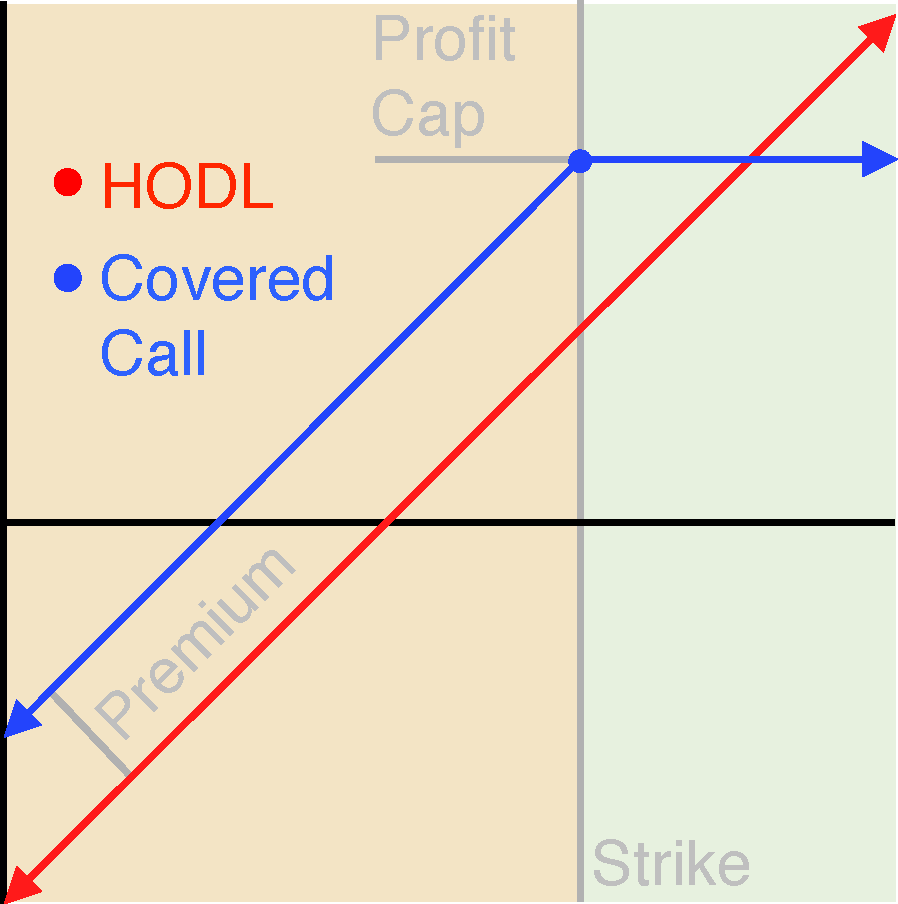
\includegraphics[width=0.5\linewidth]{coveredcall.pdf}
    \caption{The payoff of a covered call. The orange  region represents being ``out-the-money'' whereas the green region represents being ``in-the-money''. The gap between the red and blue lines represents the premium paid to the option seller. Finally, being ``at-the-money'' means the spot price is equal to the strike price, shown as the vertical grey line.}
    \label{fig:covercall}
\end{figure}

Finally, a \textit{covered call} is a structured product in which one sells a call option but also owns the underlying asset, thereby ``covering'' the call position if it is exercised (see Figure~\ref{fig:covercall}). Intuitively, selling a covered call bounds the seller's upside in return for premium. The seller is guaranteed to earn premium paid by the buyer but loses upside if the spot price exceeds the strike price. In other words, the seller's potential gains from the underlying asset appreciating is capped. As such, covered calls are not considered very risky products. A common strategy is to sell ``out-the-money'' covered calls, meaning the strike is above the current spot. Here, the seller is betting that price will not increase past the strike in return for a premium whereas the buyer has a directional view that the price will exceed the strike. One can also view a covered call as a hedge against the long position on the underlying.

\subsection{Replicating Black-Scholes Covered Calls}
\label{sec:coveredcall}

In Section~\ref{sec:rmm}, we showed a technique to derive invariants from payoff functions assuming three constraints on the payoff function. We now observe that the payoff of a covered call is indeed non-negative, concave, and 1-homogenous. In other words, there exists an invariant that replicates the covered call premium. The Primitive RMM-01\footnote{Built by the Primitive team. See \url{https://primitive.xyz/whitepaper-rmm-01.pdf}.} invariant is
\begin{equation}
    y - K\Phi(\Phi^{-1}(1-x)-\sigma\sqrt{\tau}) = k
\label{eq:invariant}
\end{equation}
where all other variables are as defined in previous sections. The marginal price can be written as $S(x) = Ke^{\Phi^{-1}(1-x)\sigma\sqrt{\tau}}e^{-\frac{1}{2}\sigma^2\tau}$.

To properly replicate covered calls with theta decay, it is important to optimally set the (swap) fee. We leave the details of fee experimentation to the RMM-01 whitepaper. Unlike Uniswap, which is primarily meant for traders to swap tokens, the primary users of RMM-01 are LPs who seek to obtain covered call payoffs. Traders on RMM-01 are dominated by arbitrageurs closing the price gap between RMM-01 and other markets such as Uniswap. Through arbitrage trades, fees accumulate to RMM-01 LPs, approximating the Black Scholes covered call premium. That is, there exists a zero-sum duality between LPs and arbitrageurs. RMMs take advantage of this duality for replication.

\section{Theta Vaults}
\label{sec:theta}

We review the design of Theta Vaults, as implemented by Ribbon Finance and similar protocols. A Theta Vault sells out-the-money covered calls every week ad infinitum.

Each week, a new round begins. Participants deposit the underlying asset into a vault. At fixed intervals throughout a round, the assets are aggregated and placed as collateral to sell covered call options. For instance, Ribbon deposits vault collateral into Opyn to mint options tokens (also called oTokens). This process is gas efficient as the vault makes a single transaction to Opyn for thousands of users at once. The call tokens are then sold for premium via a public auction (Ribbon uses Gnosis). Market makers and others can then buy the calls via auction. If the spot price exceeds the strike price, part of the vault's collateral (in Opyn) is relinquished to the buyers. Otherwise, the collateral is returned to the sellers along with the premium as yield.
A manager decides on the weekly strategy to set strike price. The manager may be an automated contract (e.g. set strike to be a percentage above current spot price using an oracle) or a privileged user who can manually set strike price.

Essentially, the yield accrued by users comes from the time value of an option, in other words Theta decay (hence the name). Users of Theta Vaults do not need to actively manage their positions. Their actions are limited to depositing and withdrawing the underlying. The amount of yield that users earn is strictly bounded by the vault's ability to find buyers within a constrained time interval. In Ribbon, Gnosis auctions are open for only one hour. Unmatched short positions produce no yield since no premium is paid. Much like orderbooks, a traditional marketplace matching buyers and sellers is difficult to run efficiently on-chain. Next, we propose an alternative design through replication.

\section{Replicating Theta Vaults}

We propose to offer Theta Vaults through selling covered calls replicated by RMM-01, as first described in \cite{sterrett2022replicating}. In short, doing so replaces the matching of buyers to sellers with rational arbitrage in an AMM pool -- a potentially more efficient design.

We begin with an overview of the mechanism followed by a thorough description of the implementation and technical details. We recommend reading the following in parallel to the solidity code on Github and technical documentation on Gitbook.

\subsection{Mechanism Overview}

The mechanism for ``Replicating Theta Vaults'' (RTV) is similar to traditional Theta Vaults with a few important distinctions. Each week the mechanism goes as follows:
\begin{figure}[h!]
    \centering
    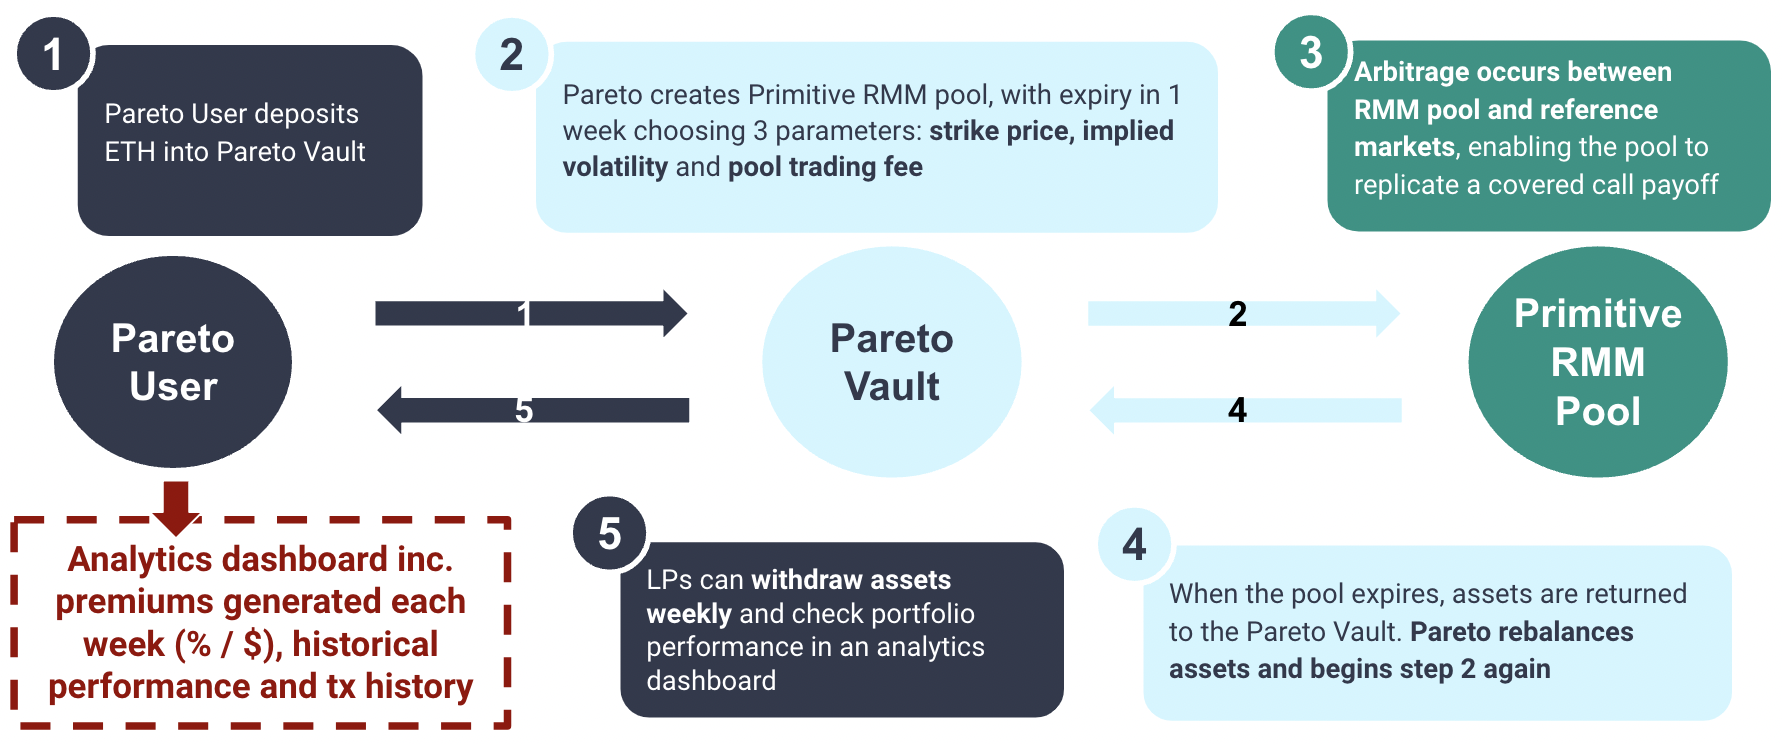
\includegraphics[width=0.8\linewidth]{userexperience.png}
    \caption{Step by Step Weekly Operations of the Pareto Vaults.}
    \label{fig:userexperience}
\end{figure}

\begin{enumerate}
    \item \textbf{User Deposits} - new users seeking yield will deposit risky assets (e.g. ETH) into the Pareto Vault. Users do not need to deposit stable assets (e.g. USDC).
    \item \textbf{Pareto creates a Primitive Pool and sets parameters} - once a week, Pareto will deposit these assets into a Primitive RMM-01 pool with a one week expiry and a set strike price, implied volatility, and Gamma (1 - Primitive pool trading fees) chosen to maximize risk-adjusted yield. In return, the pool gives LP tokens to the vault.
    \item \textbf{Premium is earned through arbitrage} - throughout the week, arbitrageurs will pay fees to swap tokens in the pool to bridge the price gap with external markets like Uniswap. The fees earnt in the pool replicate the covered call premium \cite{angeris2021replicating}, giving users the payoff of selling covered calls.
    \item \textbf{Rebalancing} - each Primitive pool requires both a risky (ETH) and stable asset (USDC), so Pareto then swaps a portion of that for USDC, using a mechanism described in Section~\ref{sec:rebalance}. When each RMM-01 pool expires, Pareto rebalances to ensure it has the correct ratio before rolling over assets.
    \item \textbf{Rollover or Withdrawal} - at the end of the week, the RMM-01 pool expires, and liquidity is either withdrawn by Pareto users or automatically rolled over to a new RMM-01 pool with an updated strike price, volatility, gamma, and an expiry date one week ahead. Much like Theta Vaults, RTVs continue to roll over ad infinitum.
\end{enumerate}

No auction nor matching process is required. Technically, there are no buyers of the covered calls as no options are being sold, their payoffs only replicated. The LP's counterparties in an RMM are arbitrageurs. As long as arbitrageurs are making rational trades to close price gaps, LPs will closely replicate the expected payoff. In other words, a single RTV can grow as large as the spot market for the risky asset in question. Whereas Theta Vaults are bounded by the amount of matched options, RTVs are not.

\subsection{Rebalancing}
\label{sec:rebalance}

Rebalancing is the swapping of vault assets to ensure they have the "optimal" ratio of risky (e.g. ETH) and stable (e.g. USDC) asset for each new round. This is necessary because RMM pools, like AMM pools require two assets. The ratio of assets each pool requires depends on the vault parameters and changes each week.

The challenge is that the ratio of risky to stable assets in the vault likely do not match the ``optimal'' ratio expected by the RMM pool.
This is due to two reasons.
First, users only deposit risky token, meaning the vault will likely own much more risky than stable asset.
Second, when an RMM-01 pool expires, assets are almost either in all risky or all stable token depending on whether the spot price is above or below the strike.

The question arises: Given the swap fees in some market, what is the right amount to swap in order to match the optimal ratio but deposit as much of the value stored in the vault as possible? We show below that this optimization problem can be cheaply solved in closed-form, meaning it is viable to perform on-chain.

\begin{figure}[h!]
    \centering
    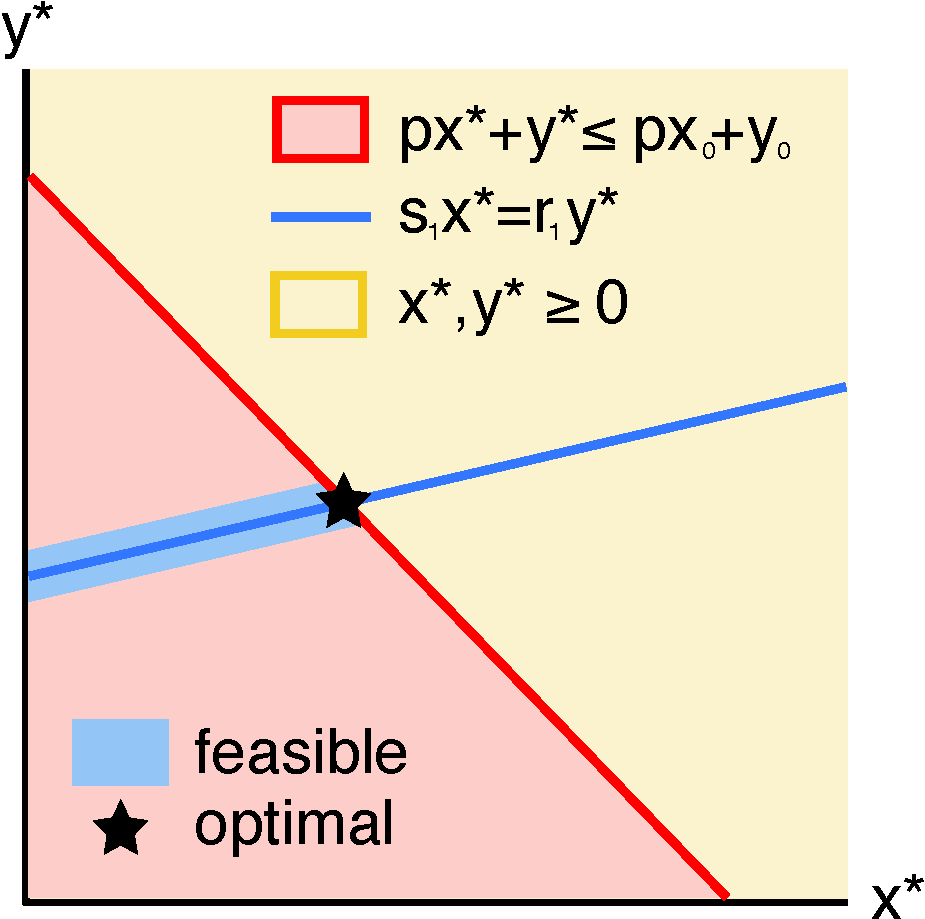
\includegraphics[width=0.5\linewidth]{rebalance.pdf}
    \caption{Illustration of the solution to the rebalancing optimization problem.}
    \label{fig:rebalance}
\end{figure}

We begin by introducing some notation. Let $p$ be the reference price of a risky token X in terms of a stable token Y. For instance, $p$ may be the exchange rate of a Uniswap-v3 or Primitive RMM-01 pool. Next, set $r_1 = 1 - \Phi(d_1)$ with $d_1$ as defined in Section~\ref{sec:options} and $\Phi$ the CDF for a standard normal. For context, $r_1$ represents the amount of risky token per liquidity token (in Primitive, this is often called referred to as \texttt{riskyPerLp}). Also, set $s_1 = K\Phi(\Phi^{-1}(1-r_1)-\sigma\sqrt{\tau}) + k$ to be the amount of stable token per liquidity token, derived using the invariant in Equation~\ref{eq:invariant}. Finally, let $(x_0, y_0)$ be the known, unbalanced  amounts of risky and stable tokens. Let $(x^*, y^*)$ be the unknown but desired balanced amounts.

We can write the rebalancing problem as the linear optimization problem:
\begin{equation}
    \begin{aligned}
        \max_{x^*, y^*}  \quad & p x^* + y^* \\
        \textrm{s.t.} \quad & s_1 x^* = r_1 y^* \\
        &  p x^* + y^* \leq p x_0 + y_0 \\
        & x^*, y^* \geq 0
    \end{aligned}
    \label{eq:rebalance}
\end{equation}
where the objective is to maximize the value (in stable token Y) captured by the optimal portfolio. The constraints, in order: (1) restrict this optimal portfolio to respect the liquidity exchange rates of the RMM-01 pool; (2) bound the optimal portfolio by the value held in the unbalanced portfolio; (3) non-negative token amounts.

\textbf{Intuition}$\quad$ Equation~\ref{eq:rebalance} is solvable off-chain using any linear optimizer but we wish to do this cheaply on-chain, meaning we cannot use iterative algorithms. The closed-form solution is best explained through visualization. Figure~\ref{fig:rebalance} illustrates the three constraints using the shaded yellow and red regions as well as the blue line. We observe that the set of feasible solutions is the intersection of the three constraints: in other words, the portion of the blue line within the red shaded area. Since the objective $p x^* + y^*$ is monotonic in both inputs, the optimal solution will be the intersection of the two lines, shown as the star.

\textbf{Solution}$\quad$ Finding the intersection between any two lines can be done in closed-form. For the rebalancing problem, we have two lines: (1) $y^* = \left(\frac{s_1}{r_1}\right)x^*$ and (2) $y^* = p(x_0 - x^*) + y_0$. Hence, the intersection is the point:
\begin{align}
    x^* &= r_1 V_0 / M \label{eq:rebalance:solution} \\
    y^* &= s_1 V_0 / M \nonumber
\end{align}
where $V_0 = px_0 + y_0$ and $M = r_1 p + s_1$.

Given the optimal portfolio $(x^*, y^*)$ using Equation~\ref{eq:rebalance:solution} and the starting portfolio $(x_0, y_0)$, it must be that either $x^* \geq x_0, y^* \leq y_0$ or $x^* \leq x_0, y^* \geq y_0$. In the first case, we can swap $x^* - x_0$ of token X on the reference market with price $p$. In the second case, we can swap $y^* - y_0$ of token Y. Finally, we can deposit $x^*, y^*$ into the RMM-01 pool at no loss.

\subsection{Vault Parameters}
\label{sec:management}

Pareto RTVs designate a special address ``keeper'' who manages the vault. Keepers are responsible for deploying new vaults each round and rolling over liquidity from the last vault. Practically, these actions will be automated as two smart contract calls.
The keeper is also responsible for choosing algorithms to decide the strike, implied volatility, and RMM-01 transaction fee: three important parameters that affect the yield users receive. 

\textbf{Implied Volatility Selection}$\quad$ The best choice for the implied volatility of a RMM-01 pool is the future realized volatility in the risky asset, which by definition, is unknown. 
Best practice is to choose implied volatility using realized volatility from recent history or recent expectations of future volatility.
There are two techniques to do so. First, one can estimate volatility from historical data. The challenges of this approach are twofold: past volatility doesn't capture expectations of future events, and, sensitivity to hyperparameter choices such as the sampling period and frequency, the price information (e.g. close-to-close vs. high-low), and the definition of volatility (e.g. Parkinson vs Rogers-Satchell). 
It is difficult to determine what is ``best'' because different choices affect the estimate significantly. 

The second approach is to back-derive volatility from a large marketplace of calls and puts using the Black-Scholes model. 
In traditional finance, this is done by VIX and emulated for DeFi through Deribit DVOL and similar services.
DVOL in particular, is an attractive choice given Deribit's large market share in DeFi options at the time of publication.
While the first approach can be done online using Uniswap-v3 TWAP prices for instance, the second approach cannot as DVOL is not available through an oracle. 

\textbf{Strike Selection}$\quad$ Having selected implied volatility $\sigma$, Pareto RTVs select the strike price on-chain. 
This is done by the keeper choosing a fixed delta value (at contract deployment; the value can be adjusted by the keeper at any time for the next round). For instance, Pareto defaults to $\Delta = 0.2$, where $\Delta = \Phi(d_1)$, from Black Scholes in \ref{sec:options}.
A larger $\Delta$ represents a more risky strategy as strike is likely closer to the current spot price. 

Given $\sigma$ and $\Delta$, the appropriate strike price under Black-Scholes can be computed by: 
\begin{equation}
  K = S \exp \left\{ \frac{\tau \sigma^2}{2} - \sigma \sqrt{\tau} \cdot \Phi^{-1}(\Delta) \right\}
  \label{eq:strike}
\end{equation}
Equation~\ref{eq:strike} can be efficiently implemented on-chain using Primitive's\newline \texttt{CumulativeNormalDistribution.sol} contract which implements the inverse CDF for a standard Normal, along with \texttt{ABDKMath64x64.sol} for exponentiation.

\textbf{Gamma Selection}$\quad$

As discussed in prior work \cite{angeris2021replicating}, replicating a covered call through an RMM fails to capture the Theta value without properly set fees.
Unfortunately, there is no known closed-form expression that maps the Black-Scholes parameters of an RMM pool to the optimal fee choice.
As such, we leverage simulations to model the relationship empirically.

Figure~\ref{fig:fee:simulation} uses \url{https://github.com/primitivefinance/rmms-py} to simulate arbitrageurs and traders interacting with an external reference market and an RMM-01 pool expiring in one week. The figure contains 400 squares, each of which is an independent simulation at a different $\left(\frac{S}{K}\right)$ ratio and a different volatility ($\sigma$). The parameter $d\tau$ represents the time between agent actions: a smaller $d\tau$ is more faithful but also more expensive. Choosing $d\tau = 1$ hour required 8 hours of computation on 1 CPU.

\begin{figure}[h!]
    \centering
    \hfill
    \begin{subfigure}[b]{0.49\textwidth}
        \centering
        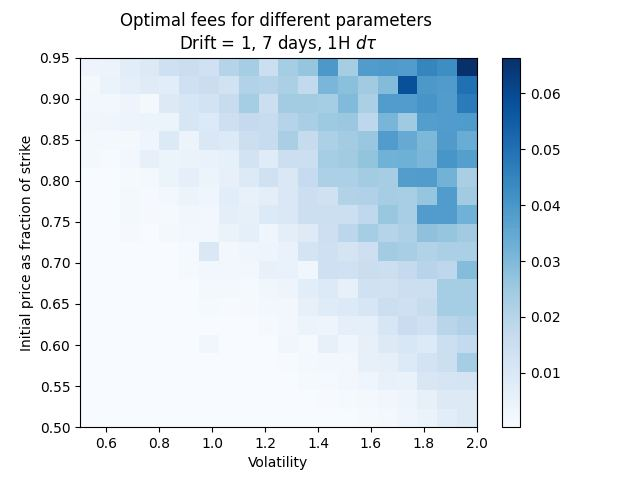
\includegraphics[width=\textwidth]{fee/simulation.png}
        \caption{Simulation}
        \label{fig:fee:simulation}
    \end{subfigure}
    \hfill
    \begin{subfigure}[b]{0.49\textwidth}
        \centering
        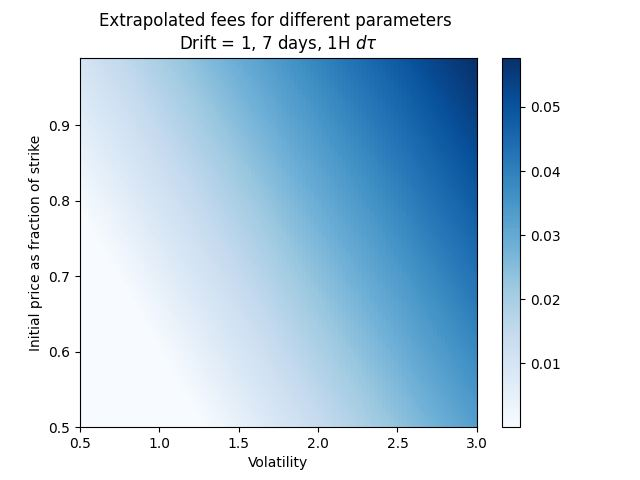
\includegraphics[width=\textwidth]{fee/reconstruction.png}
        \caption{Linear Model}
        \label{fig:fee:reconstruction}
    \end{subfigure}
    \caption{Optimal fee selection. The left subfigure shows choices of optimal fees from simulations of week-long RMM-01 pools. The right subfigure fits a linear model to the simulated data, and plots the predictions.}
    \label{fig:fee}
\end{figure}

We treat the simulation as a dataset $\{K_i, \sigma_i, 1 - \gamma_i\}_{i=1}^{400}$. Using this, we can model the function $f: (\mathbb{R}^+, \mathbb{R}^+) \rightarrow [0,1]$ from input variables (strike and volatility) to target variable (fee) using a linear regressor. In particular, we parameterize $f(K, \sigma; w_K, w_\sigma, b) = w_1 \cdot K + \sigma \cdot w_2 + b$ and choose the unknown parameters $\{w_K, w_\sigma, b\}$ by optimizing the objective
\begin{equation}
\mathcal{L}(w_K, w_\sigma, b) = \frac{1}{400}\sum_{i=1}^{400} \left(f(K_i, \sigma_i) - (1 - \gamma_i) \right)^2
\label{eq:loss}
\end{equation}
using stochastic gradient descent. We do this one-time calculation off chain using \texttt{sci-kit learn}, arriving at the optimal values:
\begin{align*}
w^*_K &= 0.01885887419001178 \\
w^*_\sigma &= 0.05105840835529893 \\
b^* &= -0.04941277762457601
\end{align*}
Now, after choosing implied volatility and deriving strike as shown in the sub-sections above, the optimal fee can be approximated efficiently on-chain through $f(K_{\textup{curr}}, \sigma_{\textup{curr}}; w^*_K, w^*_\sigma, b^*)$: three constants, two multiplications, and two additions via \texttt{ABDKMath64x64.sol}.

\textbf{Manual Override}$\quad$ Although selection is largely automated, the keeper reserves the right to manually override algorithmic choices to ensure vault success. At any point in the current round, the keeper may change the strike, implied volatility, or gamma for the \textit{next} round.

\subsection{Fee Structure}
\label{sec:fees}

Pareto RTVs take a performance fee and a management fee if and only if the vault accrued yield that round.
That is, if the value of the vault's assets after expiry is less than the value of those assets at-deposit, then no fees are taken since the user would have been better off holding onto their tokens.
The ``value'' is computed in a single token (either risky or stable) and requires an oracle for the exchange rate.
The performance fee is a percentage of the yield whereas the management fee is a percentage of the total assets in the vault. These percentages are set at deployment and can be changed only by the contract owner.

\subsection{Benefits}

Swapping options buyers for arbitrageurs, results in several potential benefits:
\begin{itemize}
    \item \textbf{Uncapped Vault Sizes} - by the nature of replication, Pareto RTVs are not reliant on demand for options from market makers.
    \item \textbf{Potentially Higher Yield} - given Pareto Vaults are not selling options during a fixed 1 hour window each week (e.g. auctions), this could increase premiums.
    \item \textbf{More Flexible Withdrawals} - in RMM pools, fees accumulate over time, rather than at a fixed point in time (e.g. an auction). Whilst in V1, we will only allow weekly withdrawals; in later versions, we will offer a flexible system for withdrawing capital - multiple times a week rather than once a week in Traditional Theta Vaults.
    \item \textbf{Potentially Favorable Legal Treatment} - since participating in an RTV is providing liquidity to AMM without a counterparty, there may be favorable legal treatment.
    \item \textbf{Blockchain outages do not have adverse effects} - RMMs are a form of AMM and have a continuous price function (unlike order books), so  a lack of liveness (e.g. Solana 2021, 2022) may not excessively adversely impact market participants.
\end{itemize}
Separately, Pareto hopes to catalyze the growth of RMMs given RMMs can be daunting for retail users: they are required to choose a strike price, expiry date, and implied volatility for their deposits. Implied volatility, in particular, is not well understood. Pareto aims to abstract away this complexity from users to help the Primitive ecosystem grow. 

\subsection{Challenges}
\label{Challenges}

Benefits aside, RTVs have their own unique challenges:
\begin{itemize}
    \item \textbf{External dependencies} - first, like regular Theta Vaults, RTVs still require strike price to be set either automatically or manually. In the case of the former, this requires an oracle. Further, creating an RMM-01 pool requires setting the implied volatility of the underlying Black-Scholes model, for which the optimal value is the true volatility of the risky asset at the current time. This can be difficult to measure and requires an oracle as well. Although RTVs no longer use oracles to determine liquidation, they still rely on oracles in vault creation and fee computation.
    \item \textbf{Rebalancing risk} - second, the solution to rebalancing in Section~\ref{sec:rebalance} would face significant slippage as the liquidity locked within the vault grows large. Potential solutions include dynamically routing swaps to find the best price in a manner similar to the 1inch protocol, or prematurely rolling liquidity over to the next pool with intentional mispricing \cite{sterrett2022replicating}. More research is needed to better understand these solutions.
    \item \textbf{Payoff replication risk} - finally, Primitive pools must achieve a minimum scale for accurate replication. We have seen that accurate replication can be achieved at very low levels of liquidity from the Primitive whitepaper using carefully chosen transaction fees. These should be even lower on Layer 2's where gas costs are significantly lower. Pareto RTVs would benefit from simulations on- and off-chain to estimate the minimum scale for proper replication of covered call premiums.
\end{itemize}

\section{Conclusion and Future Work}

We have provided a technical description for a new design of Theta Vaults built on Replicating Market Makers, aptly named Replicating Theta Vaults. RTVs provide a yield mechanism by which users replicate the premium of selling covered calls by providing liquidity to an token swap pool. The proposed approach has potential capital efficiency benefits at the cost of rebalancing costs.
An RTV protocol is currently being designed by the Pareto team.

\subsection{Roadmap}

There are two interesting directions to build on. First, covered calls are only one structured product that can be replicated by RMM-01. Others include calls, puts, binary options, strangles, condors, etc \cite{sterrett2022replicating}. By building similar vaults for other products, we will create a larger options ecosystem using replication. Second, as with most DeFi protocols, the first release of Pareto RTVs will focus on ETH and USDC. Afterwards, Pareto RTVs will look to expand to L2 chains given cheaper gas fees as well as other token pairs in top 20.

\bibliographystyle{unsrt}
\bibliography{main}

\appendix

\section{Solidity Notes}

We direct the reader to the code \url{https://github.com/pareto-xyz/pareto-theta-vault-v1} and the technical documentation \url{https://pareto-labs.gitbook.io/technical}, both of which will be kept up-to-date. We encourage developers to contribute through raising issues, making pull requests, joining the discord, or getting in touch with us directly.

\end{document}


\begin{comment}

\subsection{User Flow}

Users can take three primary actions (which are done through a frontend or an API): deposit liquidity, request a withdrawal, and complete a withdrawal.

\textbf{Deposit Liquidity}$\quad$ Users can make deposits of any size in risky token only.
The vault will handle swaps for stable tokens internally.
Upon depositing, the users tokens will remain in a ``pending'' status until the next round.
That is, the user's liquidity will \textit{not} be placed in the current vault immediately.
Once the next vault is deployed, the users pending tokens will then be locked into the underlying RMM-01 pool.

After receiving a deposit, the vault mints share tokens for the user. Pareto internally tracks share ownership and opts not to transfer them out of the contract.

\textbf{Request a Withdrawal}$\quad$ Users cannot withdraw tokens instantaneously from the vault. They must wait until the current round completes. However, users can make a request to withdraw liquidity at any point. A request must be made prior to withdrawal completion. Users must specify how many shares they wish to withdraw (default is to withdraw all).

\textbf{Complete a Withdrawal}$\quad$ After the round during which a withdrawal request is made, the user can complete a withdrawal. This will immediately transfer \textit{both} risky and stable tokens to the user's address, and burn the appropriate amount of share tokens held by the vault. Note that Pareto RTV's do not automatically convert user assets all back to risky token. Users will need to do this themselves.

There are three special users: an owner, a keeper, a fee recipient. The owner is responsible for deploying the contract, and has control over setting the keeper, fee recipient, and other key vault parameters. The keeper is responsible for managing the vault each round (see Section~\ref{sec:management}). The fee recipient receives fees for vault operation (see Section~\ref{sec:fees}).

\subsection{Vault Operations}

The vault undergoes three primary actions (both of which occur prior to every round): deployment, fee payment, and rollover.

\textbf{Deployment}$\quad$ At the end of a round, the vault prepares for the next round by deploying a new RMM-01 pool with a new strike price, implied volatility, and gamma set by the keeper based on current market prices (see Section~\ref{sec:management}). Only a small amount of capital is deposited into this new pool. Afterwards, liquidity is extracted from the current RMM-01 pool and transferred to the vault's ownership. % does ownership mean contract?

\textbf{Fee Payment}$\quad$ Immediately following deployment, analysis is done to check if the vault made a profit. If so, a performance fee and a management are transferred from the vault to the chosen fee recipient. If the vault took a loss, no fees are taken.

\textbf{Rollover}$\quad$ The risky and stable assets owned by the vault are rebalanced through swaps using the Uniswap-v3 router (see Section~\ref{sec:rebalance}), then placed in the newly deployed RMM-01 pool in exchange for LP tokens. A new round begins.

\end{comment}

% EXTRA

% Beyond this, there are several important design elements:
% \begin{itemize}
%     \item Deposit and withdrawal times: Pareto Vaults will deposit and withdraw from Primitive RMM-01 pools twice a week - each Tuesday and Friday at [5pm UTC]. Any user that wishes to withdraw at that time, must input their request with the Pareto protocol beforehand. Limiting withdrawals to twice weekly improves gas efficiency. As we expand to L2s, we hope to offer more frequent deposit and withdrawal opportunities.
%     \item Vault Tokens: Initially, we will offer only a ETH-USDC vault. Once Pareto launches on mainnet, we will expand our offering to other Top 20 tokens.
%     \item Multi Token Deposits: In the Alpha, users will have to deposit ETH and USDC, this creates friction for users and over time, we plan to remove the need for users to deposit USDC.
%     \item Receipt Tokens: Users will not receive vault tokens by default, however we will reconsider this over time.
%     \item Rebalancing: When a RMM-01 vault expires, all assets will be either the risky asset (e.g. ETH) or the stable asset (e.g. USDC). However, when depositing in a new pool, one needs both risky and stable assets. Our initial approach to handling this is initiating mispriced pools. This is discussed in further detail in \ref{Challenges} [Add more data].
%     \item Expiry Date Selection: Pools will expire each Friday at [5pm UTC].
%     \item Strike Selection: [TBD]
%     \item Implied Volatility Selection: [TBD]
%     \item Pool Fees Selection: [TBD]
% \end{itemize}
